%===============================================================================
% $Id: ifacconf.tex 19 2011-10-27 09:32:13Z jpuente $  
% Template for IFAC meeting papers
% Copyright (c) 2007-2008 International Federation of Automatic Control
%===============================================================================
\documentclass{ifacconf}

\usepackage{graphicx}      % include this line if your document contains figures
\usepackage{natbib}        % required for bibliography
 
\usepackage{pgfplots} 
\pgfplotsset{compat=newest} 
\pgfplotsset{plot coordinates/math parser=false} 
\newlength\figureheight 
\newlength\figurewidth 


\usepackage{caption}
\captionsetup[figure]{name=Fig.,labelfont={sf,bf},textfont=sl,labelsep=quad}
\usepackage[caption=false,font=footnotesize,labelformat=simple]{subfig}
%===============================================================================
\begin{document}
\begin{frontmatter}

\title{Stable Non-Convex MPC via Convex Feasibility Set Algorithm for Motion Planning\thanksref{footnoteinfo}} 
% Title, preferably not more than 10 words.

\thanks[footnoteinfo]{This work was supported by National Science Foundation (Award \#1734109).}

\author[First]{ Jessica Leu} 
\author[Second]{ Changliu Liu} 
\author[First]{ Masayoshi Tomizuka}

\address[First]{ University of California,
Berkeley, CA 94720 USA\\ \tt jess.leu24@berkeley.edu, tomizuka@me.berkeley.edu}
\address[Second]{ Stanford University, CA 94305 USA\\ \tt  changliuliu@stanford.edu}


\begin{abstract}                % Abstract of not more than 250 words.
Real-time, safe and stable motion planning in cluttered environments remains challenging due to the non-convexity of the problem. This paper investigates MPC-based motion planning. As there are many local optima due to non-convexity, it is important to guarantee stability of the non-convex MPC such that the trajectories will not jump around multiple local optima. In order to tackle stability, a notion of $M$-stability is introduced in this paper, which guarantees finite convergence (at least $M$ steps) of the planned trajectories. With such notion, we verify the stability of the non-convex MPC which implements the convex feasible set algorithm (CFS) at every MPC step through extensive simulations. The $M$-stability analysis provides a tractable tool to understand dynamics of non-convex MPC.
 

\end{abstract}

\begin{keyword}
Motion planning, Non-convex MPC, Optimization, Convexification, Stability.
\end{keyword}

\end{frontmatter}
%===============================================================================

\section{Introduction}
Examining the vibrant development in motion planning for autonomous driving and robotics, it is no doubt that this is the core of improving mobility in the future. One of the important and impactful application that uses these techniques is automated guided vehicles (AGVs) serving in factories (Wu et al., 2004). In this paper, assuming that a low level controller is in hand, we focus on optimization-based AGV-trajectory planning method and its stability analysis. Although the environment in a factory is not as dynamic as driving scenarios, safety and efficiency still need to be guaranteed throughout the planning and executing process (Wang et al., 2008; Oleari et al., 2014).

With the above performance requirements, Model predictive control (MPC) (Rawlings, 1999) is a framework that fits the need. MPC has been wildly used both in academia research and in industrial applications. Its ability to handle input and state constraints makes it a popular method to deal with motion planning problem. 
This paper focuses on a two-dimensional motion planning problem. %The motion planning environment (the state space) this work focuses on is a 2-dimensional plan. 
The existence of obstacles makes it non-convex. Therefore, the problem is an non-convex MPC problem that has non-convex state constraints. 

MPC implementation in industries has been around for more then 2 decades. Though being aware of the importance of stability, industrial proponents of MPC don't usually address it theoretically. On the other hand, research in academia has put more effort on stability. Usually, stability can be guaranteed by modifying prediction horizon, adding terminal cost, adding terminal equality constraint, or using terminal constraint set instead (Mayne et al., 2000). These methods have been found useful when developing stabilizing model predictive controllers. However, the literature that utilized these techniques often consideres MPC tracking problem as regulating problem, which is regulating around a steady-state point. Imagine a car driving on a road, the terminal goal might be too far away that we instead make the car to reach to a series of interim goals until reaching the terminal goal. In this sense, the problem is a full tracking problem (Limon et al., 2006) that does not only track a point. This  is the type of problem studied in this paper.

Several literature had focused on MPC that handles target changes. One way of analyzing stability in these cases is to ensure feasibility, which is often sufficient to enable a simple guarantee of closed loop stability for the controller (Bocciaa et al., 2014; Dughman et al., 2015; Zhanga et al., 2016). One commonly seen application for non-regulating MPC problem is among autonomous driving car (Borrelli, 2006). In the literature, stability is guaranteed by setting stability boundary for the control system, i.e., stability is quantified at several vehicle speeds. Generally, most of the stability analysis is still done by considering a regulation problem. Asymptotic stability can be guaranteed when feasibility is held and the cost-to-go is decreasing step by step.

One major problem of applying these stability analyzing methods to this work is that the problem here is non-convex. The fact that MPC problem is non-convex makes the close loop stability hard to be analyzed. Some work focused on MPC problem with non-convex cost function using sequential convex optimization method (Hovgaard et al., 2012). Although the control result is promising, the difficulty of ensuring stability for non-convex MPC is also mentioned in the literature. 
Analyzing stability of non-convex MPC problem remains challenging. Even the notion of stability is still not clear for non-convex MPC.
%It is clear that there is still a lot of effort that could be made in analyzing stability for non-convex MPC problem. 

In this paper, we first introduce a new notion of stability called $M$-stability and then analyze the properties of a non-convex MPC via the convex feasible set algorithm (CFS) (Liu et al., 2018).  The relationships among the optimal trajectories generated at different steps will be examined, so as to  guarantee that the robot trajectory will not experience sudden jumps when being executed. Simulation studies are performed to test the performance of the implementing CFS  algorithm in MPC framework. Finally, the stability properties is analyzed using the proposed method.

The remainder of the paper is organized as follows. Section 2 provides problem formulation. Section 3 discusses the simulation setup. Section 4 shows simulation results. Section 5 concludes the paper.

\section{Problem Formulation}

\begin{figure}[htbp]
\begin{center}
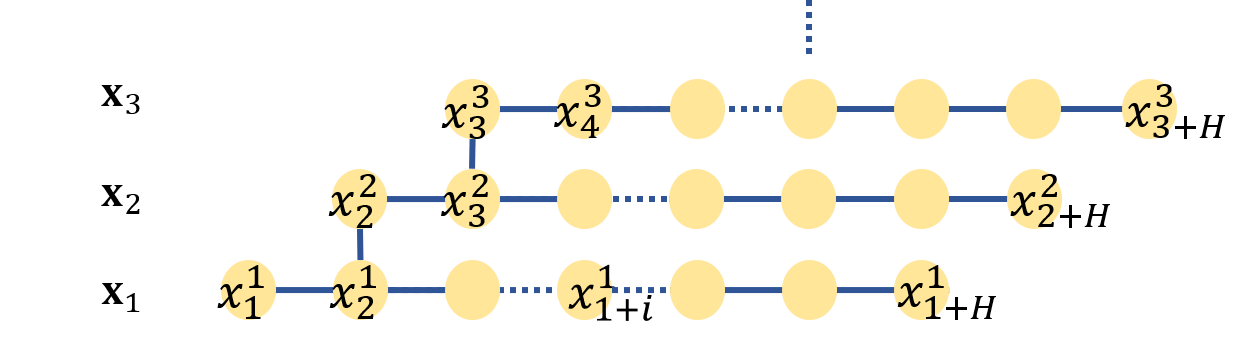
\includegraphics[width=8cm]{src/MPCstruc.png}
\caption{The execution structure of MPC}
\label{fig: mpc}
\end{center}
\end{figure}

\subsection{Problem and Notations}
In MPC, at each time step, $t$, a planned trajectory will be calculated. This trajectory is denoted as $\mathbf{x}_{t=k}=\mathbf{x}_{k} := [x_k, x_{k+1},x_{k+2},\cdots,x_{k+H}]$ where $x_k$ is called the $k^{th}$ action location that contains the $x$ and $y$ coordinate of the robot's location in 2-dimensional Cartesian space at time step $t=k$. Note that $x_k$ correspond to the current position at time step $t=k$. The trajectory will then be executed and the robot will go to $x_{k+1}$, the $k+1^{th}$ action location, which is the planned action location for the robot at time step $t=k+1$. The time range between two time step is a constant denoted as $\Delta t$. After reaching the next action location, the robot will again plan a new trajectory and repeat the process. To avoid confusion, the current time step can also be marked as superscript in some cases , e.g., $x_{k+1}^k$ means the planned action location $x_{k+1}$ at time step $t=k$.

At time step $k=t$, given the current state $x_k$, the following optimization needs to be solved to obtain $\mathbf{x}_k$,
\begin{eqnarray}
&\min_{\mathbf{x}_{k}} & J(\mathbf{x}_k)\\
&s.t.& x_{k+i}\in\Gamma,\forall i=1,\ldots,H
\end{eqnarray}

\begin{assum}[Cost]
The cost function is convex and regular, and has the following form
\begin{eqnarray}
J(\mathbf{x}_k) = \sum_{i=1}^{H} \|x_{k+i}\|_{Q}^2 + \sum_{i=1}^{H-1} \|x_{k+i}-x_{k+i+1}\|_R^2
\end{eqnarray}
\end{assum}

\begin{assum}[Constraint]
Where the state constraint $\Gamma$ is non-convex and its complement is a collection of disjoint convex sets, i.e., the each of the obstacle is itself convex.
\end{assum}

Note that the problem is time-invariant. The final trajectory is $[x_k^k,x_{k+1}^{k+1},\ldots]$, which is equivalent to $[x_{k}^{k-1},x_{k+1}^{k},\ldots]$ (Fig.1). As the problem is non-convex, it is possible that the planned trajectories calculated at different time steps enter into different local optima, hence the stability is hard to characterize . 

\subsection{$M$-stable Stability Analysis}
In this paper, we propose a new way of analyzing stability. Under the condition that the environment in the future time step is not going to change much, we say that the non-convex MPC is $M$-stable if $\|x_{k}^t-x_k^{t-1}\|\leq \|x_k^{t-1}-x_k^{t-2}\|$ for all $k$ and $k-M< t\leq k$ (Fig.2). Note that the problem is always $1$-stable, since $\|x_{k}^t-x_k^{t-1}\|=0$. We say that a action location, $x_{k}$, has $M$-stable property if the above inequality holds for the last $M$ time steps at $x_{k}$.  The notation implies that the planned state $x_k$ would have smaller and smaller change on each predicted action location between consecutive time steps after time step $k-M$. This result can also be expressed as saying the output solutions are all close to one local optimum after time step $k-M$. 

Having such property is good for the robot. $M$-stable guarantees that the action location will not change much, and therefore, guarantees smoothness of the output trajectory and the robot system will not experience sudden change. Moreover, since the planned trajectory is usually tracked by a low-level tracking controller, the larger the $M$ is, the smoother the control commend would be.

\begin{figure}[htbp]
\begin{center}
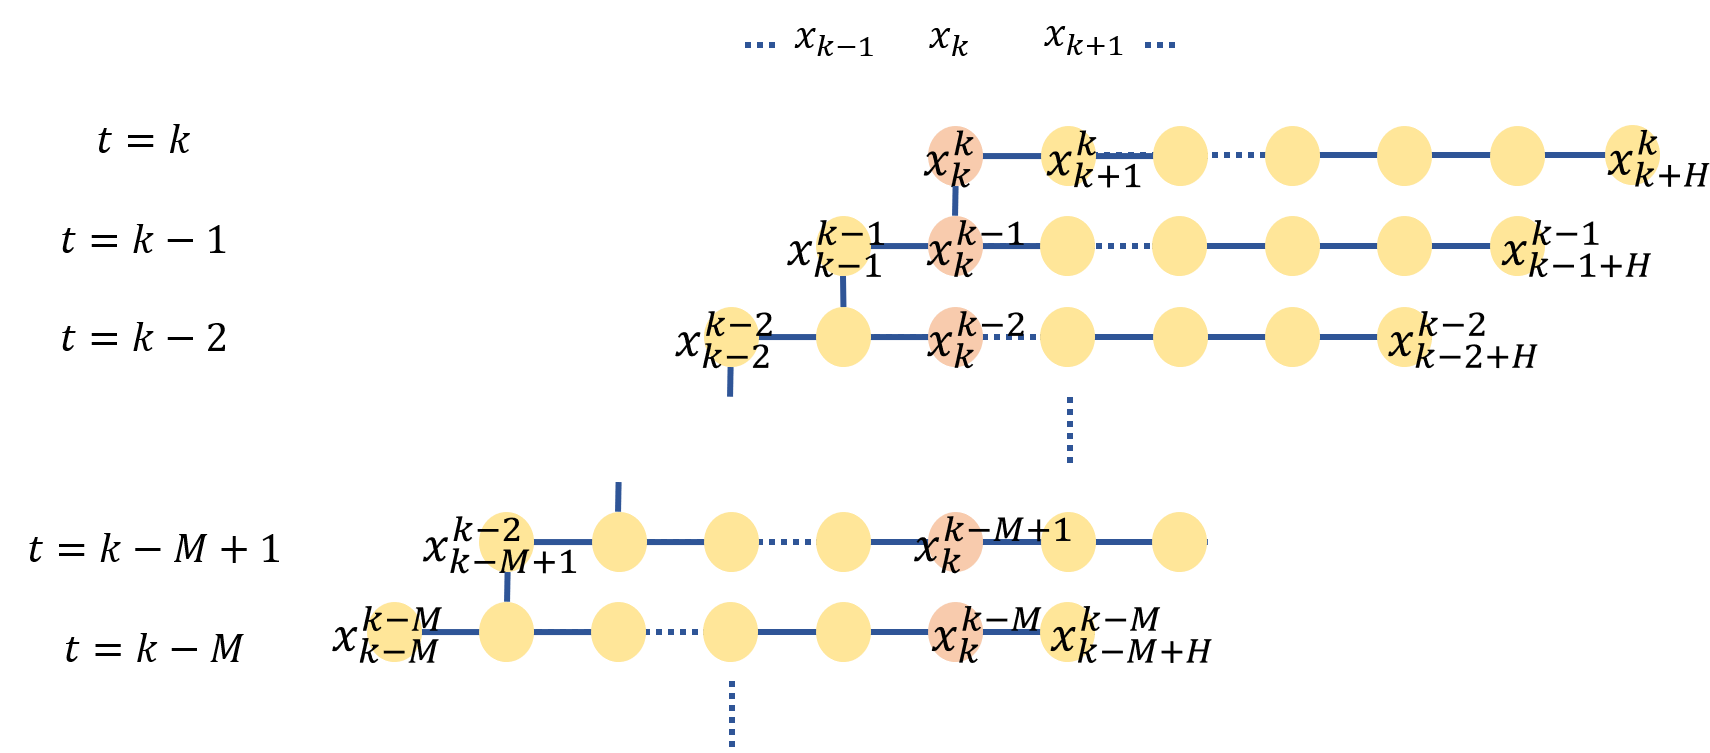
\includegraphics[width=9.5cm]{src/Mstable.png}
\caption{The pink-orange-color circles are the planned action location tested for M-stable for one $k$. Note that the inequality needs to be hold for all $k$.}
\label{fig: mpc}
\end{center}
\end{figure}


\subsection{The Convex Feasible Set Algorithm}
Because the problem we are solving has non-convex state constrains, the problem is a non-convex MPC problem. Here we solve the optimization problem at each MPC step using the convex feasible set algorithm (CFS), which iteratively solve a sequence of sub-problems of the original non-convex problem using convex constraints, e.g., convex feasible set. The CFS algorithm in the MPC structure uses the previous solution, the planned action locations as a reference. The convex feasible set for a reference point $x_r$ is computed as $\mathcal{F}(x_r) = \{x:A(x_r)x\leq b(x_r)\}$ where $A(x_r)$ is a matrix and $b(x_r)$ is a column vector. 
At time step $k+1$, the reference is set as $\mathbf{x}_{k+1}^{r}=[x_{k+1}^{k},x_{k+2}^{k},\ldots,x_{k+H}^k, x_{k+H+1}^*]$ where
\begin{eqnarray}
x_{k+H+1}^* = \arg\min_{x_{k+H+1}} \|x_{k+H+1}\|_Q^2\\+\|x_{k+H}^k-x_{k+H+1}\|_R^2
\end{eqnarray}
If $x_{k+H+1}^*\in\Gamma$, then the optimal solution $\mathbf{x}_{k+1}^o = \mathbf{x}_{k+1}^r$.  If $x_{k+H+1}^*\notin\Gamma$, denote the feasible solution as 
\begin{eqnarray}
\bar{x}_{k+H+1} = \arg\min_{x_{k+H+1}\in\Gamma} \|x_{k+H+1}\|_Q^2\\
+\|x_{k+H}^k-x_{k+H+1}\|_R^2
\end{eqnarray}
Moreover, denote $\mathbf{x}_{k+1}^{u}:=[x_{k+1}^{k},x_{k+2}^{k},\ldots,x_{k+H}^k, \bar x_{k+H+1}]$. 

Then the optimal solution $\mathbf{x}_k^{o}$ at step $k$ satisfies that
\begin{eqnarray}
\mathbf{x}_k^{o} = \arg\min_{x_{k+i}\in \mathcal{F}(x_{k+i}^o)}J(\mathbf{x}_k)
\end{eqnarray}
Note that $J(\mathbf{x}_k^{r})\leq J(\mathbf{x}_k^{o})\leq J(\mathbf{x}_k^{u})$. 
The executed trajectory is from those $\mathbf{x}_k^{o}$ for different $k$.


\subsection{Stability with CFS}
In this paper, we will show that the system is stable through simulation. We will leave the theoretical proof as future work. But here we sketch the procedures. First, we can show that at two consecutive plans, the difference between the early state should be strictly smaller than the difference between any future state, i.e., $\|x_{k+i}^{k+1}-x_{k+i}^k\|<\lambda\|x_{k+i+1}^{k+1}-x_{k+i+1}^k\|$ for some $\lambda<1$. Then we can show that the state is bounded and the difference between the same state at different time steps keeps decreasing.
%the KKT condition is satisfied, i.e.,
%\begin{eqnarray}
%2Qx_{k+i}^k +2R(2x_{k+i}^k-x_{k+i-1}^k-x_{k+i+1}^k) + \eta_{k+i}^k A(x_{k+i}^k) \nonumber\\
%= 0,\forall i=1,\ldots,H
%\end{eqnarray}
%where $\eta_{k+i}^k$ is the Lagrangian multiplier such that $\eta_{k+i}^k\geq 0$ and $\eta_{k+i}^k= 0$ if and only if $A(x_{k+i}^k)x_{k+i}^k= b(x_{k+i}^k)$.
%
%Hence
%\begin{eqnarray}
%(Q+2R)(x_{k+i}^{k+1}-x_{k+i}^k)=R(x_{k+i-1}^{k+1}-x_{k+i-1}^k)\\+R(x_{k+i+1}^{k+1}-x_{k+i+1}^k)-(\eta_{k+i}^{k+1} A(x_{k+i}^{k+1})-\eta_{k+i}^k A(x_{k+i}^k))
%\end{eqnarray}
%
%Claim that $\|x_{k+i}^{k+1}-x_{k+i}^k\|<\lambda\|x_{k+i+1}^{k+1}-x_{k+i+1}^k\|$ for some $\lambda<1$.

\section{Simulation setup}
\subsection{Optimization problem setup}
The simulation scenario in this work is similar to that of mobile robots operating in factories. The state $x_{k} = (x,y)$, the action location, contains the $x$ and $y$ coordinate of the robot's location in 2-dimensional Cartesian space. The detailed robot dynamics are not considered in the planner.  It is assumed that a low-level controller can track the planned trajectories without any error. In the simulations, we solve the optimization problem in an MPC framework and generate the next 20 optimal planned action location at each time step. The initial point of the optimization problem, the current state, is denoted as $x_0(t)$,The optimization problem at time step $t=k$ is formulate as below. 

\begin{eqnarray}
&\min_{\mathbf{x}_{k}} & J(\mathbf{x}_k)\\
&s.t.& x_{k+i}\in\Gamma,\forall i=1,\ldots,H\\
&&         x_{k}=x_0(k)
\end{eqnarray}

Where $H$ is set to be 20 and the current state is measured and assigned to the first entry of $\mathbf{x}_{k}$. Note that $x_{k}$ need not to be in the feasible set. Considering that there is disturbance in the real world, perfect tracking is usually impossible. This is the reason why we might have infeasible initial point. The advantage of CFS algorithm is its ability to cope with infeasible initial point. $\Gamma$ is a non-convex state constraint as discussed in Assumption 1.

The low-level tracking controller on the robot can then track the first planned action location, and then, the robot will calculate the optimal output again. Note that the simulation assumes perfect tracking.

The cost function of the optimization problem shown below is designed to fit the task and the environment that the robot is in.

\begin{eqnarray}
J(\mathbf{x}_k) = C_1\|\mathbf{D}\mathbf{x}_k-\mathbf{d}\|_{2}^2 + C_2 \|\mathbf{R}\mathbf{x}_k-\mathbf{v}_{ref}\|_2^2 +\|\mathbf{A}\mathbf{x}_{k}\|_2^2  
\end{eqnarray}

Where the first term penalizes the robot's deviation from a reference line so that the robot output trajectory is not too irregular. In this work, the reference is set to be a horizontal line, $y=0$. The second term penalize the speed profile of the planned trajectory with regard to a constant speed so that the robot will be time efficient. Here, the speed reference is set to be a constant speed going along the positive $x$-axis. The third term penalizes the acceleration of the output trajectory so that it will be smooth.  

\subsection{Simulation scenarios}

To test our algorithm, three kinds of scenarios will be considered. The first one is a static scenario, i.e., every environment information is known, while the other two are dynamic scenarios, i.e., the robot will experience changes in the environment.

\subsubsection{single static obstacle}
In this scenario, there is  only one static obstacle. This is the scenario as discussed in section 2, where the optimization problem is time invariant. $M$-stable property, and some other stability analysis is done under this setting.

\subsubsection{initially unknown static obstacle}
In this scenario, the robot does not know all the obstacle location at the beginning, and has only limited ``eye sight," i.e., only the information of the environment within the range starting from 20 meters ahead to its current position. The robot is expected to execute this MPC motion planning and adjust it's planned trajectory to avoid collision once it ``sees" the obstacle.

\subsubsection{initially unknown moving obstacle}
In this scenario, there exists a moving obstacle, which is not observed by the robot at the beginning. Once the robot sees this obstacle, it also gets the information of the obstacle's dynamics, and therefore, is able to predict the future position of the obstacle and conduct planning accordingly. 

In the following section, the simulation results of these three scenarios are shown, and the stability features are discussed using the proposed methods.



\section{Simulation result and stability discussion}

The goal for the robot is to move in the direction of $x$-plus alond a line, $y=0$, while maintaining a constant speed which also points to $x$-plus direction. 
\subsection{single static obstacle}
The simulation result is shown in Fig.3. We can see that the robot successfully avoid collision while maintain its movement along the horizontal line which it is supposed to track after passing by the obstacle. It is clear from the figure that the last several action locations planned at each time step are one on top of another. This can be taken as indication of stability. 

Fist, in order to test the stability of CFS, we show that in between two consecutive plans, the difference between the early state should be strictly smaller than the difference between any future state. In Fig.4, from $k=20$ to $k=26$ the trend holds. After $k=26$, the difference starts to decrease and then hold at a constant. This is because the robot is simply moving along a straight line after $k=26$ and therefore every action location after $k=26$ planned in one time step has equal distance. Thus, the difference between two time step is constant for these action locations. 




Fig.5 shows the largest possible number $M$ for $M$-stable at each action location, i.e., the largest $M$ that  $\|x_{k}^t-x_k^{t-1}\|\leq \|x_k^{t-1}-x_k^{t-2}\|$ and $k-M< t\leq k$ hold for each $x_k$. From the figure, we  notice that $M$ is higher near the current position. (The figure shows simulation result that runs for 20 time step, therefore the current position is at the $20^{th}$ action location). Note from Fig.3, the last several action locations planned from different time step are almost the same, the decrease of $M$ for action location after $k^{th}$ might caused by numerical reasons. In other words, since the difference between action locations are already very small, there is no need to check $M$-stable for these locations. If we decrease the sampling time to one fifth of the original, i.e, $\Delta t_{new}=0.2\Delta t_{original}$, the number $M$ for each action location holds the same for a longer period of time as shown in Fig.7. Concluding from the figures, robot under this scenario can be considered as $5$-stable.

 

\begin{figure}[htbp]
\begin{center}
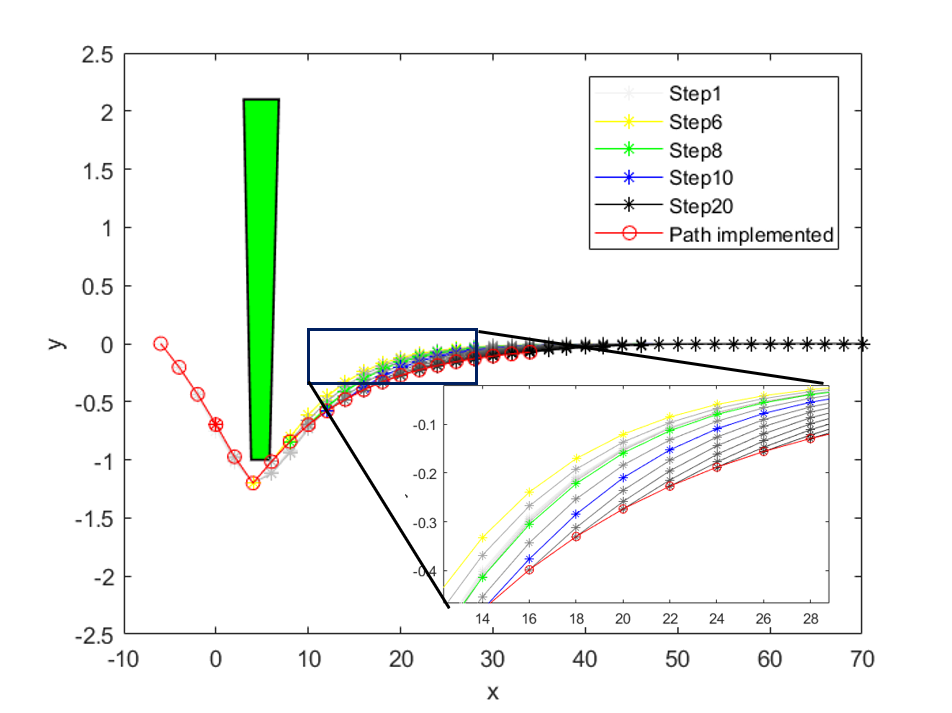
\includegraphics[width=10cm]{src/1_1.png}
\caption{Simulation result for single static obstacle. The planned trajectory is marked by gray-star-line of which the gray-color gets darker as time step increases. Several specific time steps are marked with colors shown in legend.  }
\label{fig: mpc}
\end{center}
\end{figure}

\begin{figure}[htbp]
\begin{center}
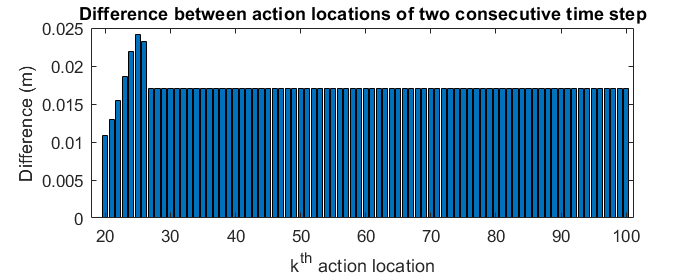
\includegraphics[width=8cm]{src/1_1_4.png}
\caption{Simulation result for single static obstacle.}
\label{fig: mpc}
\end{center}
\end{figure}

\begin{figure}[htbp]
\begin{center}
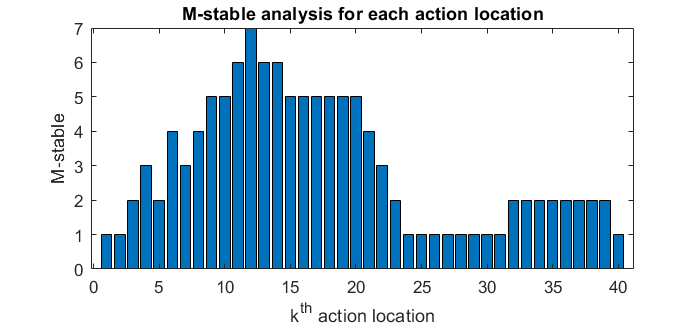
\includegraphics[width=8cm]{src/1_2_M-stable.png}
\caption{Largest possible number $M$ for $M$-stable for each action location.}
\label{fig: mpc}
\end{center}
\end{figure}



\begin{figure}[htbp]
\begin{center}
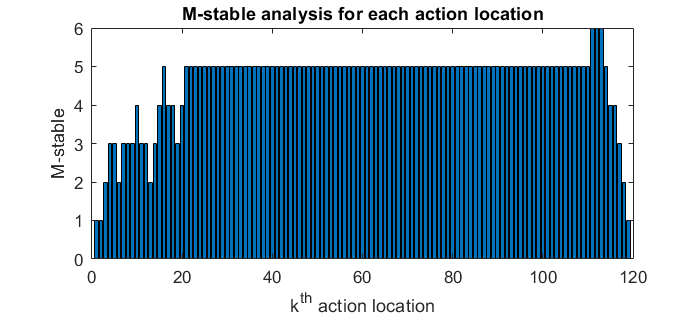
\includegraphics[width=8cm]{src/1_2_M-stable_2.png}
\caption{Largest possible number $M$ for $M$-stable for each action location with increased sampling rate.}
\label{fig: mpc}
\end{center}
\end{figure}



\begin{figure}[htbp]
\begin{center}
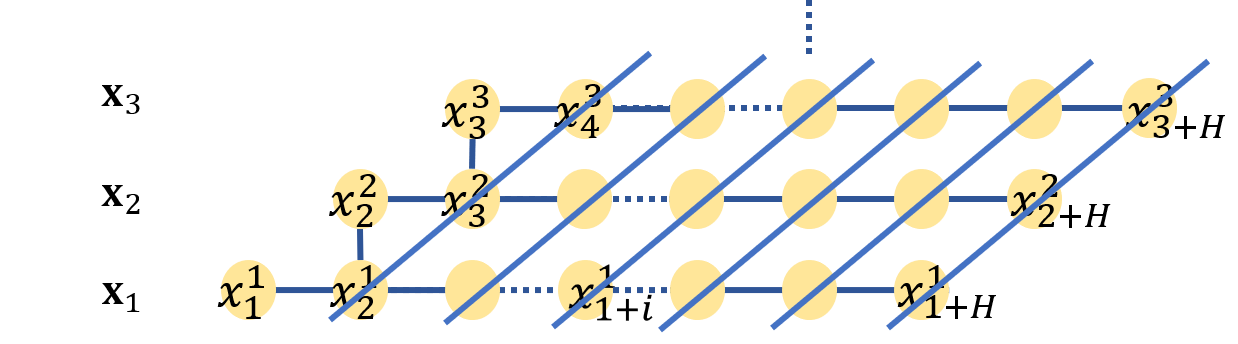
\includegraphics[width=8cm]{src/1_3_path.png}
\caption{Illustration of path$_k$ (the diagonal lines).}
\label{fig: mpc}
\end{center}
\end{figure}

\begin{figure}[htbp]
\begin{center}
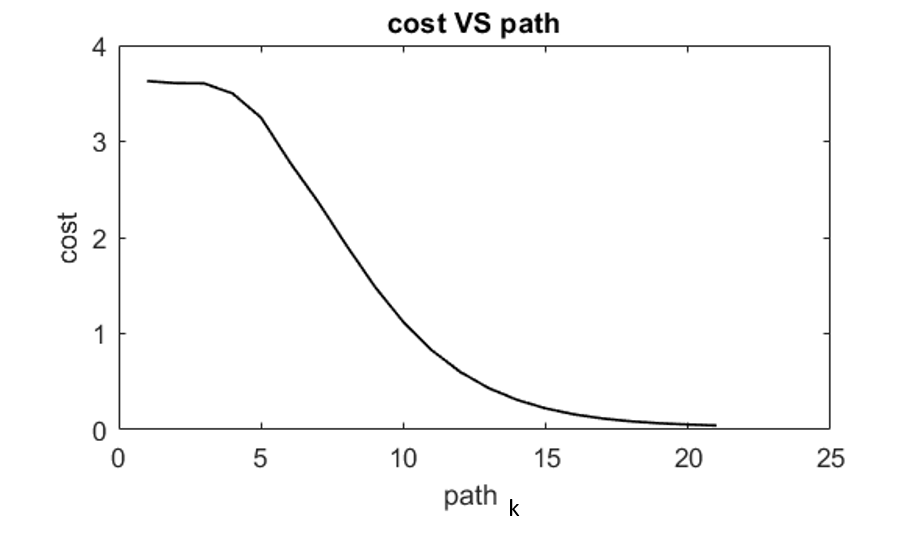
\includegraphics[width=8cm]{src/1_3.png}
\caption{Cost VS path.}
\label{fig: mpc}
\end{center}
\end{figure}

Another way to analyze stability is to look at the cost change. Define path$_k$ as $\mathbf{x}_{k}^{p} := [x_{k}^{k-1},x_{k+1}^{k},\ldots]$ (Fig.7). Increase of the index $k$ means the path is starting further and further away from disturbance, i.e., the obstacle, which located close to the robot's initial location. Therefore, it is expected that the cost will decrease as $k$ increases, which indicates that the robot is stably doing better and better according to what the cost function wants it to do. This expectation meets perfectly with Fig.8. 

\subsection{initially unknown static obstacle}

The result of this scenario is shown in Fig.9. At the beginning, the robot does not know there exists the third obstacle on the right. After detecting the third obstacle, the robot corrects its planned trajectory to avoid the obstacle and completes its intention successfully.

The $M$-stable stability analysis discussed previously can also be applied to this scenario even though the environment is changing. Since the stability analysis strategy of this work looks close into the relation among planned action locations, i.e., every point in the trajectories, the analysis can still be done although the planned location changes a lot due to environment changes. This directly demonstrate the strength of the proposed $M$-stable analysis. The result for $M$-stable is shown in Fig.10. Notice that this simulation runs for 30 time steps, we can see that the numbers for $M$ are all around 6 when $k$ is close to 30. The decrease of $M$ after $k=30$ is again caused by numerical reason as discussed previously.     




\begin{figure}[htbp]
\begin{center}

\subfloat[]{
  % This file was created by matlab2tikz.
%
%The latest updates can be retrieved from
%  http://www.mathworks.com/matlabcentral/fileexchange/22022-matlab2tikz-matlab2tikz
%where you can also make suggestions and rate matlab2tikz.
%
\definecolor{mycolor1}{rgb}{0.96667,0.96667,0.96667}%
\definecolor{mycolor2}{rgb}{0.93333,0.93333,0.93333}%
\definecolor{mycolor3}{rgb}{0.86667,0.86667,0.86667}%
\definecolor{mycolor4}{rgb}{0.83333,0.83333,0.83333}%
%
\begin{tikzpicture}

\begin{axis}[%
width=3.036in,
height=1.698in,
at={(0.677in,0.229in)},
scale only axis,
xmin=-10,
xmax=65,
ymin=-11,
ymax=11,
axis background/.style={fill=white},
legend style={legend cell align=left, align=left, draw=white!15!black}
]

\addplot[area legend, line width=1.0pt, draw=black, fill=green, forget plot]
table[row sep=crcr] {%
x	y\\
3	2.1\\
6.8	2.1\\
5.8	-1\\
3.8	-1\\
}--cycle;

\addplot[area legend, line width=1.0pt, draw=black, fill=green, forget plot]
table[row sep=crcr] {%
x	y\\
23	0.1\\
26.8	0.1\\
26.8	-10\\
23	-10\\
}--cycle;
\addplot [color=mycolor1, mark=asterisk, mark options={solid, mycolor1}]
  table[row sep=crcr]{%
-6	0\\
-4.30573668770685	-0.121230126216136\\
-2.87630513826835	-0.28418834756381\\
-1.46522555388652	-0.484790237321453\\
-0.0554176999716383	-0.723563785594289\\
1.35430202722899	-0.995883299879068\\
2.76401564753985	-1.2777178813988\\
4.17372884466345	-1.5\\
5.58344201246159	-1.5\\
6.99315517822756	-1.29295766765565\\
8.4028683438527	-1.03555026771578\\
9.81258150946808	-0.794624647748671\\
11.2222946750828	-0.59349103192322\\
12.6320078406974	-0.435624414091703\\
14.0417210063121	-0.316458735507208\\
15.4514341719267	-0.228997186341746\\
16.8611473375414	-0.166272084701486\\
18.2708605031561	-0.12223411313811\\
19.6805736687707	-0.0918639150066664\\
21.0902868343854	-0.0708643147212668\\
22.5	-0.0550302398687101\\
};
\addlegendentry{Step1}

\addplot [color=blue, mark=o, mark options={solid, blue}, forget plot]
  table[row sep=crcr]{%
-4.30573668770685	-0.121230126216136\\
};
\addplot [color=mycolor2, mark=asterisk, mark options={solid, mycolor2}, forget plot]
  table[row sep=crcr]{%
-4.30573668770685	-0.121230126216136\\
-2.65651671917057	-0.266952161175341\\
-1.31114544737889	-0.464964150352054\\
0.013170114912306	-0.70749239953417\\
1.33602658619104	-0.985773136994679\\
2.65878194728953	-1.27354421516906\\
3.98153030178702	-1.5\\
5.30427817075024	-1.5\\
6.62702600606755	-1.29282873264247\\
7.94977383905331	-1.03520785774391\\
9.2725216718775	-0.793992794718195\\
10.5952695046905	-0.592481476028427\\
11.9180173375027	-0.434124066569769\\
13.2407651703149	-0.314323612051515\\
14.563513003127	-0.226055432324677\\
15.8862608359392	-0.162344804033397\\
17.2090086687514	-0.117193007923362\\
18.5317565015635	-0.0857635006292117\\
19.8545043343757	-0.0642212327973607\\
21.1772521671878	-0.0493865997739125\\
22.5	-0.0382227526693035\\
};
\addplot [color=blue, mark=o, mark options={solid, blue}, forget plot]
  table[row sep=crcr]{%
-2.65651671917057	-0.266952161175341\\
};
\addplot [color=white!90!black, mark=asterisk, mark options={solid, white!90!black}, forget plot]
  table[row sep=crcr]{%
-2.65651671917057	-0.266952161175341\\
-1.05114258111082	-0.44613497572038\\
0.21240322267365	-0.687325900883055\\
1.45226145371996	-0.971638946531279\\
2.69047821433809	-1.26738288773159\\
3.92858122648582	-1.5\\
5.16667635624085	-1.5\\
6.40477093977214	-1.29276530604793\\
7.64286548545193	-1.03503894564045\\
8.88096002850875	-0.793679847744095\\
10.1190545713838	-0.59197862529895\\
11.3571491142463	-0.433370836583504\\
12.5952436571078	-0.313239825476144\\
13.8333381999694	-0.224538782830126\\
15.0714327428309	-0.160273892455568\\
16.3095272856924	-0.114442475156813\\
17.5476218285539	-0.0822448936533275\\
18.7857163714154	-0.0599763048043718\\
20.023810914277	-0.0447841171138046\\
21.2619054571385	-0.0343551244244603\\
22.5	-0.0265185122240942\\
};
\addplot [color=blue, mark=o, mark options={solid, blue}, forget plot]
  table[row sep=crcr]{%
-1.05114258111082	-0.44613497572038\\
};
\addplot [color=mycolor3, mark=asterisk, mark options={solid, mycolor3}, forget plot]
  table[row sep=crcr]{%
-1.05114258111082	-0.44613497572038\\
0.947814819670018	-0.81134502698654\\
2.945869111991	-1.21686777768904\\
4.94386082188336	-1.5\\
6.94184819502056	-1.37599981301129\\
8.93983526763667	-1.10380804161612\\
10.9378223194521	-0.799469727853893\\
12.9358093701787	-0.507766240499674\\
14.9337964259187	-0.239822875139846\\
16.9317835554403	0.00674332366700078\\
18.9297717497832	0.235617871842776\\
20.9277753102518	0.441303293810504\\
22.9260006147228	0.594926657297048\\
24.927425841103	0.61951883609815\\
26.9289724786052	0.583602733701758\\
28.9290796554676	0.494471171211914\\
30.9290870824696	0.398992678773523\\
32.9290875971363	0.316138762996624\\
34.929087632801	0.251243584883324\\
36.9290876352733	0.202813736117701\\
38.9290876354565	0.165026293813502\\
};
\addplot [color=blue, mark=o, mark options={solid, blue}, forget plot]
  table[row sep=crcr]{%
0.947814819670018	-0.81134502698654\\
};
\addplot [color=mycolor4, mark=asterisk, mark options={solid, mycolor4}]
  table[row sep=crcr]{%
0.947814819670018	-0.81134502698654\\
2.94723374530955	-1.19056291357689\\
4.94614933931302	-1.5\\
6.94503005409931	-1.38584799703101\\
8.94390835187264	-1.11578298813507\\
10.9427864821751	-0.810232153962354\\
12.941664601163	-0.516090613117848\\
14.9405427235599	-0.245446523172548\\
16.9394209067027	0.00366776350884273\\
18.9382999672517	0.234727319088293\\
20.9371916894455	0.44199646200136\\
22.9362661280816	0.596107938395995\\
24.9379772934867	0.619015838060864\\
26.9397561252479	0.580393907341798\\
28.9398793924043	0.4882001855657\\
30.9398879344105	0.389244711143201\\
32.9398885263432	0.302546636883444\\
34.9398885673622	0.233791580119787\\
36.9398885702047	0.182509335089464\\
38.9398885704017	0.145276522890386\\
40.9398885704163	0.116569014281613\\
};
\addlegendentry{Step5}

\addplot [color=blue, mark=o, mark options={solid, blue}, forget plot]
  table[row sep=crcr]{%
2.94723374530955	-1.19056291357689\\
};
\addplot [color=white!80!black, mark=asterisk, mark options={solid, white!80!black}, forget plot]
  table[row sep=crcr]{%
2.94723374530955	-1.19056291357689\\
4.94695163354805	-1.5\\
6.94642515413918	-1.38578448503687\\
8.94588174086197	-1.11561753906816\\
10.9453371541412	-0.80993539271986\\
12.9447924863577	-0.515635799474801\\
14.9442478166075	-0.244811019731421\\
16.9437031994023	0.00449106933474043\\
18.943159346068	0.235701796196104\\
20.942626516316	0.442982254755956\\
22.9422527646352	0.59674331495702\\
24.9441746214064	0.618487034824828\\
26.9461293302121	0.578324508381646\\
28.9462647850658	0.484489354832561\\
30.9462741716391	0.383648368383868\\
32.9462748220975	0.294740959050428\\
34.9462748671721	0.223490906985536\\
36.9462748702956	0.169713623024239\\
38.9462748705121	0.130786356704104\\
40.9462748705271	0.103025685232069\\
42.9462748705282	0.0817921654039152\\
};
\addplot [color=blue, mark=o, mark options={solid, blue}, forget plot]
  table[row sep=crcr]{%
4.94695163354805	-1.5\\
};
\addplot [color=black!8!mycolor4, mark=asterisk, mark options={solid, black!8!mycolor4}, forget plot]
  table[row sep=crcr]{%
4.94695163354805	-1.5\\
6.94664469025044	-1.21470383616901\\
8.9460718700153	-0.905050683170402\\
10.9454806254061	-0.616417947359808\\
12.9448881043103	-0.359440709528344\\
14.9442954985333	-0.129760902088701\\
16.9437029413654	0.081302862826938\\
18.9431111737102	0.279611996928819\\
20.942530805381	0.460585453378963\\
22.9421149377656	0.596993746667083\\
24.9440729311739	0.616295537032931\\
26.9460666682596	0.578683000281083\\
28.946204827644	0.485076372836287\\
30.9462144016323	0.383301058378714\\
32.946215065078	0.292844298440329\\
34.9462151110526	0.219687558893756\\
36.9462151142384	0.16382010088551\\
38.9462151144592	0.122891448386582\\
40.9462151144745	0.0938295230783457\\
42.9462151144756	0.0733510378181918\\
44.9462151144757	0.0577729493336347\\
};
\addplot [color=blue, mark=o, mark options={solid, blue}, forget plot]
  table[row sep=crcr]{%
6.94664469025044	-1.21470383616901\\
};
\addplot [color=black!12!mycolor4, mark=asterisk, mark options={solid, black!12!mycolor4}, forget plot]
  table[row sep=crcr]{%
6.94664469025044	-1.21470383616901\\
8.94641692202166	-0.965267894629919\\
10.9459918590008	-0.689785927415296\\
12.9455531243545	-0.425643472049886\\
14.9451134459312	-0.18140652561228\\
16.9446737543677	0.0456883339575248\\
18.9442348160474	0.258903811566242\\
20.9438068128941	0.452278504442167\\
22.9435366164178	0.596985426868887\\
24.9455436815925	0.617249782683278\\
26.9475772704741	0.577984984343555\\
28.9477181914561	0.483477378654109\\
30.947727956814	0.38107573216735\\
32.947728633521	0.290007922104333\\
34.9477286804145	0.216114957289613\\
36.9477286836641	0.159324873066676\\
38.9477286838893	0.117311397210423\\
40.9477286839049	0.087170318025758\\
42.947728683906	0.0660680522928613\\
44.947728683906	0.0513319076165083\\
46.947728683906	0.0401688495151028\\
};
\addplot [color=blue, mark=o, mark options={solid, blue}, forget plot]
  table[row sep=crcr]{%
8.94641692202166	-0.965267894629919\\
};
\addplot [color=white!70!black, mark=asterisk, mark options={solid, white!70!black}, forget plot]
  table[row sep=crcr]{%
8.94641692202166	-0.965267894629919\\
10.9461678406125	-0.740314302686911\\
12.9457030029846	-0.48609261853155\\
14.945223217798	-0.234161784682464\\
16.9447424492299	0.00707846211515625\\
18.944262369187	0.235591180824513\\
20.9437932561426	0.442621743258917\\
22.9434824760509	0.596894884052978\\
24.9454565567754	0.618625539858187\\
26.9474596431353	0.577904987296564\\
28.9475984503935	0.482667622153166\\
30.9476080692773	0.37984235177019\\
32.9476087358342	0.288430749762385\\
34.9476087820243	0.214149106343575\\
36.9476087852252	0.156857153533965\\
38.947608785447	0.11420201334118\\
40.9476087854623	0.0833063564045567\\
42.9476087854634	0.0614624943244575\\
44.9476087854635	0.0463233183092771\\
46.9476087854635	0.035820937883647\\
48.9476087854635	0.0278896944515099\\
};
\addplot [color=blue, mark=o, mark options={solid, blue}, forget plot]
  table[row sep=crcr]{%
10.9461678406125	-0.740314302686911\\
};
\addplot [color=black!20!mycolor4, mark=asterisk, mark options={solid, black!20!mycolor4}]
  table[row sep=crcr]{%
10.9461678406125	-0.740314302686911\\
12.9458715905997	-0.52870641406243\\
14.9453187299428	-0.283377346233429\\
16.9447481401062	-0.0331139540022462\\
18.9441770878074	0.209932937341541\\
20.9436170589878	0.431659949764771\\
22.9432173330777	0.596807118906925\\
24.945130975877	0.62024156127871\\
26.9470791171054	0.577940807717131\\
28.9472141168477	0.482002713279988\\
30.9472234718833	0.378872393852647\\
32.9472241201563	0.287298717161373\\
34.9472241650795	0.212865252607834\\
36.9472241681925	0.155360739804499\\
38.9472241684082	0.112395131608544\\
40.9472241684232	0.0810797961906124\\
42.9472241684242	0.0587314815299306\\
44.9472241684243	0.0430964561748202\\
46.9472241684243	0.0323410592498915\\
48.9472241684243	0.0249166212861049\\
50.9472241684243	0.0193228993324973\\
};
\addlegendentry{Step10}

\addplot [color=blue, mark=o, mark options={solid, blue}, forget plot]
  table[row sep=crcr]{%
12.9458715905997	-0.52870641406243\\
};
\addplot [color=black!24!mycolor4, mark=asterisk, mark options={solid, black!24!mycolor4}, forget plot]
  table[row sep=crcr]{%
12.9458715905997	-0.52870641406243\\
14.9451985365373	-0.3196306618581\\
16.9439425389186	-0.0723631852295447\\
18.9426470355146	0.181827259450315\\
20.9413616417801	0.418751559095684\\
22.9402623440377	0.596496165131011\\
24.9418513285124	0.622620104220936\\
26.9435186897847	0.579263116929798\\
28.9436342324049	0.482693476192677\\
30.9436422391263	0.379162423096829\\
32.9436427939656	0.287305818740509\\
34.9436428324142	0.212638627436899\\
36.9436428350785	0.154905229088508\\
38.9436428352632	0.111684968703611\\
40.943642835276	0.0800684988178036\\
42.9436428352768	0.0573641187810465\\
44.9436428352769	0.0413327479269348\\
46.9436428352769	0.0302036042413337\\
48.9436428352769	0.0225903818980173\\
50.9436428352769	0.0173545555298355\\
52.9436428352769	0.013416778662304\\
};
\addplot [color=blue, mark=o, mark options={solid, blue}, forget plot]
  table[row sep=crcr]{%
14.9451985365373	-0.3196306618581\\
};
\addplot [color=white!60!black, mark=asterisk, mark options={solid, white!60!black}, forget plot]
  table[row sep=crcr]{%
14.9451985365373	-0.3196306618581\\
16.944326279901	-0.102833315855688\\
18.9426994458641	0.153297750382067\\
20.9410344474729	0.404506109999756\\
22.9395706433443	0.596409095312835\\
24.9410623203771	0.624746045984467\\
26.9426555593661	0.579355192905859\\
28.9427659655573	0.481973563314904\\
30.9427736163411	0.378200059370587\\
32.9427741465151	0.286338967889468\\
34.9427741832544	0.211740778951174\\
36.9427741858004	0.154070485512274\\
38.9427741859768	0.110869989331473\\
40.942774185989	0.0792125665209127\\
42.9427741859898	0.0563995304112827\\
44.9427741859899	0.0401937593576906\\
46.9427741859899	0.0288417877226991\\
48.9427741859899	0.0210073616102868\\
50.9427741859899	0.0156709104995867\\
52.9427741859899	0.0120114832900739\\
54.9427741859899	0.00926309530683742\\
};
\addplot [color=blue, mark=o, mark options={solid, blue}, forget plot]
  table[row sep=crcr]{%
16.944326279901	-0.102833315855688\\
};
\addplot [color=black!32!mycolor4, mark=asterisk, mark options={solid, black!32!mycolor4}, forget plot]
  table[row sep=crcr]{%
16.944326279901	-0.102833315855688\\
18.9431407569108	0.128673991815372\\
20.9409440501817	0.388361229479561\\
22.9389042166147	0.596310938700271\\
24.9401502276384	0.62731883534518\\
26.9415340274567	0.579797846445256\\
28.9416299202062	0.48153051605228\\
30.9416365652565	0.377464414998988\\
32.9416370257365	0.28557120298535\\
34.9416370576463	0.211035763481208\\
36.9416370598575	0.153443306061891\\
38.9416370600108	0.110298743171075\\
40.9416370600214	0.0786587692135949\\
42.9416370600221	0.0558174359023984\\
44.9416370600222	0.0395351768128955\\
46.9416370600222	0.0280610908362228\\
48.9416370600222	0.0200716045792873\\
50.9416370600222	0.0145823899670535\\
52.9416370600222	0.0108556745178722\\
54.9416370600222	0.00830581583326776\\
56.9416370600222	0.0063928161711595\\
};
\addplot [color=blue, mark=o, mark options={solid, blue}, forget plot]
  table[row sep=crcr]{%
18.9431407569108	0.128673991815372\\
};
\addplot [color=black!36!mycolor4, mark=asterisk, mark options={solid, black!36!mycolor4}, forget plot]
  table[row sep=crcr]{%
18.9431407569108	0.128673991815372\\
20.9417923449589	0.372509100660308\\
22.9395169944582	0.596330426847445\\
24.9406561844006	0.629574286934603\\
26.9419479462995	0.579519708764522\\
28.9420374611257	0.480317787369886\\
30.9420436642071	0.376054745064965\\
32.9420440940601	0.284270354340394\\
34.9420441238475	0.209940976223734\\
36.9420441259117	0.152556960329485\\
38.9420441260547	0.109584288572163\\
40.9420441260647	0.0780667669182742\\
42.9420441260654	0.0552965619574338\\
44.9420441260654	0.0390361602798664\\
46.9420441260654	0.0275381220195619\\
48.9420441260654	0.0194843810051483\\
50.9420441260655	0.0139021135872207\\
52.9420441260655	0.01008001386436\\
54.9420441260655	0.00749175410331937\\
56.9420441260655	0.00572392585854391\\
58.9420441260655	0.0043987487374454\\
};
\addplot [color=blue, mark=o, mark options={solid, blue}, forget plot]
  table[row sep=crcr]{%
20.9417923449589	0.372509100660308\\
};
\addplot [color=gray, mark=asterisk, mark options={solid, gray}, forget plot]
  table[row sep=crcr]{%
20.9417923449589	0.372509100660308\\
22.9398853455116	0.596381601037896\\
24.9410307402831	0.629579059476723\\
26.9423048635693	0.579457984110389\\
28.942393156098	0.480236664937572\\
30.9423992744781	0.375973800464111\\
32.9423996984616	0.28419548329865\\
34.9423997278422	0.209871389680634\\
36.9423997298782	0.152488533458297\\
38.9423997300193	0.109510977693679\\
40.9423997300291	0.0779810090047666\\
42.9423997300297	0.0551891586627134\\
44.9423997300297	0.0388959666618652\\
46.9423997300297	0.0273518442340341\\
48.9423997300297	0.0192369390644474\\
50.9423997300297	0.0135784152557529\\
52.9423997300297	0.00966978063782195\\
54.9423997300296	0.00700056687311991\\
56.9423997300296	0.00519652701883541\\
58.9423997300296	0.00396597274370978\\
60.9423997300296	0.00304413215512191\\
};
\addplot [color=blue, mark=o, mark options={solid, blue}, forget plot]
  table[row sep=crcr]{%
22.9398853455116	0.596381601037896\\
};

\addplot[area legend, line width=1.0pt, draw=black, fill=green, forget plot]
table[row sep=crcr] {%
x	y\\
43	10\\
49.8	10\\
49.8	-1\\
43.5	-1\\
}--cycle;
\addplot [color=black!50!mycolor2, mark=asterisk, mark options={solid, black!50!mycolor2}, forget plot]
  table[row sep=crcr]{%
22.9398853455116	0.596381601037896\\
24.9427030343211	0.60314119204023\\
26.9476333084854	0.577804756588279\\
28.9479749601747	0.438691417926482\\
30.9479986355066	0.255612658346385\\
32.9480002761287	0.054462678784065\\
34.9480003898184	-0.160680562732834\\
36.9480003976967	-0.395458873093158\\
38.9480003982426	-0.657297565470826\\
40.9480003982804	-0.947379200393772\\
42.948000398283	-1.24814293138903\\
44.9480003982832	-1.50000000000009\\
46.9480003982833	-1.55650117000911\\
48.9480003982833	-1.5000000000001\\
50.9480003982833	-1.27852382004827\\
52.9480003982833	-1.02721088669519\\
54.9480003982833	-0.802354888779395\\
56.9480003982833	-0.622117438523328\\
58.9480003982833	-0.486851677540312\\
60.9480003982833	-0.388290720154033\\
62.9480003982833	-0.312177498609529\\
};
\addplot [color=blue, mark=o, mark options={solid, blue}, forget plot]
  table[row sep=crcr]{%
24.9427030343211	0.60314119204023\\
};
\addplot [color=black!50!mycolor3, mark=asterisk, mark options={solid, black!50!mycolor3}, forget plot]
  table[row sep=crcr]{%
24.9427030343211	0.60314119204023\\
26.9457172580495	0.578295798015645\\
28.9459261337206	0.439319476250036\\
30.9459406080519	0.256229389332701\\
32.9459416110135	0.055019843464577\\
34.9459416804537	-0.160186054095426\\
36.9459416852039	-0.395014364107568\\
38.9459416854714	-0.656893050853408\\
40.9459416854285	-0.947024548775977\\
42.9459416853681	-1.247893045364\\
44.9459416853639	-1.50000000000013\\
46.9459416853637	-1.5570714491935\\
48.9459416853637	-1.5000000000002\\
50.9459416853637	-1.27475323782431\\
52.9459416853637	-1.01782004506852\\
54.9459416853637	-0.786108426954408\\
56.9459416853637	-0.598246173770949\\
58.9459416853637	-0.455480336924727\\
60.9459416853637	-0.351693867302397\\
62.9459416853637	-0.277485382556323\\
64.9459416853637	-0.220657799411877\\
};
\addplot [color=blue, mark=o, mark options={solid, blue}, forget plot]
  table[row sep=crcr]{%
26.9457172580495	0.578295798015645\\
};
\addplot [color=white!40!black, mark=asterisk, mark options={solid, white!40!black}, forget plot]
  table[row sep=crcr]{%
26.9457172580495	0.578295798015645\\
28.9457172580495	0.418496727815201\\
30.9457172580495	0.230615840272563\\
32.9457172580495	0.031505108083899\\
34.9457172580495	-0.17912921039126\\
36.9457172580495	-0.40891790534083\\
38.9457172580495	-0.666112494670364\\
40.9457172580495	-0.952221548208361\\
42.9457172580495	-1.24990524315403\\
44.9457172580495	-1.5\\
46.9457172580495	-1.55705250803135\\
48.9457172580495	-1.5\\
50.9457172580495	-1.27287457522497\\
52.9457172580495	-1.0129336535084\\
54.9457172580495	-0.777383177420373\\
56.9457172580495	-0.584977629669864\\
58.9457172580495	-0.437174798263567\\
60.9457172580495	-0.328484947896797\\
62.9457172580495	-0.251116093871448\\
64.9457172580495	-0.19651250226529\\
66.9457172580495	-0.154945265672115\\
};
\addplot [color=blue, mark=o, mark options={solid, blue}, forget plot]
  table[row sep=crcr]{%
28.9457172580495	0.418496727815201\\
};
\addplot [color=black!56!mycolor4, mark=asterisk, mark options={solid, black!56!mycolor4}, forget plot]
  table[row sep=crcr]{%
28.9457172580495	0.418496727815201\\
30.9457172580496	0.26103075814587\\
32.9457172580496	0.0685822198501429\\
34.9457172580496	-0.145641293084201\\
36.9457172580496	-0.3827487849812\\
38.9457172580496	-0.648009184992007\\
40.9457172580496	-0.941630437075622\\
42.9457172580496	-1.24560045197784\\
44.9457172580496	-1.5\\
46.9457172580496	-1.55784459540449\\
48.9457172580496	-1.5\\
50.9457172580496	-1.27159515043971\\
52.9457172580496	-1.01000054196475\\
54.9457172580496	-0.772412032836895\\
56.9457172580496	-0.577528503893271\\
58.9457172580496	-0.426780724421257\\
60.9457172580496	-0.314790913249377\\
62.9457172580496	-0.234221237135159\\
64.9457172580496	-0.177704384702491\\
66.9457172580496	-0.138188394559281\\
68.9457172580496	-0.10823651722304\\
};
\addplot [color=blue, mark=o, mark options={solid, blue}, forget plot]
  table[row sep=crcr]{%
30.9457172580496	0.26103075814587\\
};
\addplot [color=black!60!mycolor4, mark=asterisk, mark options={solid, black!60!mycolor4}]
  table[row sep=crcr]{%
30.9457172580496	0.26103075814587\\
32.9457172580496	0.0962876021708383\\
34.9457172580496	-0.112495528512046\\
36.9457172580496	-0.353821398085587\\
38.9457172580496	-0.626839363752318\\
40.9457172580496	-0.928853760857085\\
42.9457172580496	-1.24032517227614\\
44.9457172580496	-1.50000000000001\\
46.9457172580496	-1.55871009555787\\
48.9457172580496	-1.50000000000002\\
50.9457172580497	-1.27076865415868\\
52.9457172580497	-1.00828334222462\\
54.9457172580497	-0.769645932634311\\
56.9457172580497	-0.573468077884848\\
58.9457172580497	-0.421108911262053\\
60.9457172580497	-0.307163506220837\\
62.9457172580497	-0.224378371443793\\
64.9457172580497	-0.165721975434564\\
66.9457172580497	-0.125008237508507\\
68.9457172580497	-0.0967363072508379\\
70.9457172580497	-0.0753758262055403\\
};
\addlegendentry{Step20}

\addplot [color=blue, mark=o, mark options={solid, blue}, forget plot]
  table[row sep=crcr]{%
32.9457172580496	0.0962876021708383\\
};
\addplot [color=white!30!black, mark=asterisk, mark options={solid, white!30!black}, forget plot]
  table[row sep=crcr]{%
32.9457172580496	0.0962876021708383\\
34.9457172580496	-0.0862172385143777\\
36.9457172580496	-0.323479944471226\\
38.9457172580496	-0.602074031338828\\
40.9457172580495	-0.91306470798812\\
42.9457172580495	-1.23361177661394\\
44.9457172580495	-1.5\\
46.9457172580495	-1.55975412947941\\
48.9457172580495	-1.5\\
50.9457172580495	-1.27012161055854\\
52.9457172580495	-1.00713044113224\\
54.9457172580496	-0.767975501177934\\
56.9457172580496	-0.571167392831865\\
58.9457172580496	-0.417991358975491\\
60.9457172580496	-0.302990310093519\\
62.9457172580496	-0.218895081209088\\
64.9457172580496	-0.158739901839429\\
66.9457172580496	-0.116584272198706\\
68.9457172580496	-0.087550472273578\\
70.9457172580496	-0.0674924832985665\\
72.9457172580496	-0.0523746683695731\\
};
\addplot [color=blue, mark=o, mark options={solid, blue}, forget plot]
  table[row sep=crcr]{%
34.9457172580496	-0.0862172385143777\\
};
\addplot [color=black!68!mycolor4, mark=asterisk, mark options={solid, black!68!mycolor4}, forget plot]
  table[row sep=crcr]{%
34.9457172580496	-0.0862172385143777\\
36.9457172580495	-0.29755714363535\\
38.9457172580495	-0.574128688481032\\
40.9457172580495	-0.893231522896236\\
42.9457172580495	-1.22472450708648\\
44.9457172580495	-1.5\\
46.9457172580495	-1.56110538959235\\
48.9457172580495	-1.5\\
50.9457172580495	-1.26948249631751\\
52.9457172580495	-1.0061618995294\\
54.9457172580495	-0.766771559251552\\
56.9457172580495	-0.569701858378487\\
58.9457172580495	-0.416164921544543\\
60.9457172580495	-0.300654162484696\\
62.9457172580495	-0.215867837743744\\
64.9457172580495	-0.154833712901695\\
66.9457172580495	-0.111662261600824\\
68.9457172580495	-0.0816536086089081\\
70.9457172580495	-0.0611061647681606\\
72.9457172580495	-0.0469662650659349\\
74.9457172580495	-0.0363287083204365\\
};
\addplot [color=blue, mark=o, mark options={solid, blue}, forget plot]
  table[row sep=crcr]{%
36.9457172580495	-0.29755714363535\\
};
\addplot [color=black!75!mycolor2, mark=asterisk, mark options={solid, black!75!mycolor2}, forget plot]
  table[row sep=crcr]{%
36.9457172580495	-0.29755714363535\\
38.9457172580496	-0.548103995874345\\
40.9457172580496	-0.868896439509084\\
42.9457172580496	-1.21262423571996\\
44.9457172580496	-1.5\\
46.9457172580496	-1.56292912009079\\
48.9457172580496	-1.5\\
50.9457172580496	-1.26872546763997\\
52.9457172580496	-1.0051345666749\\
54.9457172580496	-0.765661883084489\\
56.9457172580497	-0.56854438320201\\
58.9457172580497	-0.414913531060478\\
60.9457172580497	-0.299216895403285\\
62.9457172580497	-0.214123476662963\\
64.9457172580497	-0.152643038960321\\
66.9457172580497	-0.108885663101855\\
68.9457172580497	-0.0781908088681367\\
70.9457172580497	-0.0569849136970165\\
72.9457172580497	-0.0425293541142381\\
74.9457172580497	-0.0326114287548648\\
76.9457172580497	-0.025160785659951\\
};
\addplot [color=blue, mark=o, mark options={solid, blue}, forget plot]
  table[row sep=crcr]{%
38.9457172580496	-0.548103995874345\\
};
\addplot [color=white!20!black, mark=asterisk, mark options={solid, white!20!black}, forget plot]
  table[row sep=crcr]{%
38.9457172580496	-0.548103995874345\\
40.9457172580495	-0.843959297554692\\
42.9457172580495	-1.1963603136356\\
44.9457172580495	-1.5\\
46.9457172580495	-1.56537263199079\\
48.9457172580495	-1.5\\
50.9457172580495	-1.26776263082935\\
52.9457172580495	-1.00389498022226\\
54.9457172580495	-0.764428231662428\\
56.9457172580495	-0.567399270646097\\
58.9457172580495	-0.413842464858124\\
60.9457172580495	-0.298158296065245\\
62.9457172580495	-0.212991441288835\\
64.9457172580495	-0.151337319755243\\
66.9457172580495	-0.107298145247786\\
68.9457172580495	-0.076216739075082\\
70.9457172580495	-0.0545498994507411\\
72.9457172580495	-0.0396508709087984\\
74.9457172580495	-0.0295293085519518\\
76.9457172580495	-0.0226010570300069\\
78.9457172580495	-0.0174021509826229\\
};
\addplot [color=blue, mark=o, mark options={solid, blue}, forget plot]
  table[row sep=crcr]{%
40.9457172580495	-0.843959297554692\\
};
\addplot [color=black!80!mycolor4, mark=asterisk, mark options={solid, black!80!mycolor4}, forget plot]
  table[row sep=crcr]{%
40.9457172580495	-0.843959297554692\\
42.9457172580496	-1.17766400642021\\
44.9457172580496	-1.5\\
46.9457172580496	-1.56817865061168\\
48.9457172580496	-1.5\\
50.9457172580496	-1.2666765067678\\
52.9457172580496	-1.00252361836127\\
54.9457172580496	-0.763108259301063\\
56.9457172580496	-0.566239937862917\\
58.9457172580496	-0.412846268168552\\
60.9457172580497	-0.29728019331843\\
62.9457172580497	-0.21216614042671\\
64.9457172580497	-0.150490537920829\\
66.9457172580497	-0.106350732399807\\
68.9457172580497	-0.075087442059055\\
70.9457172580497	-0.0531621060641259\\
72.9457172580497	-0.0379507686505322\\
74.9457172580497	-0.0275283680412478\\
76.9457172580497	-0.0204667724288746\\
78.9457172580497	-0.0156418341024076\\
80.9457172580497	-0.0120243953723512\\
};
\addplot [color=blue, mark=o, mark options={solid, blue}, forget plot]
  table[row sep=crcr]{%
42.9457172580496	-1.17766400642021\\
};
\addplot [color=black!84!mycolor4, mark=asterisk, mark options={solid, black!84!mycolor4}, forget plot]
  table[row sep=crcr]{%
42.9457172580496	-1.17766400642021\\
44.9457172580496	-1.5\\
46.9457172580496	-1.56817968627602\\
48.9457172580496	-1.5\\
50.9457172580496	-1.26666920533388\\
52.9457172580496	-1.00250463890986\\
54.9457172580495	-0.763073291214543\\
56.9457172580495	-0.566183530153349\\
58.9457172580495	-0.41276085238805\\
60.9457172580495	-0.297155119720696\\
62.9457172580495	-0.211986623882907\\
64.9457172580495	-0.150236519035052\\
66.9457172580495	-0.105995823638318\\
68.9457172580495	-0.0745984349277023\\
70.9457172580495	-0.0525001122993462\\
72.9457172580495	-0.0370762264441343\\
74.9457172580495	-0.0264143608245566\\
76.9457172580495	-0.0191292976987131\\
78.9457172580495	-0.0142035025303436\\
80.9457172580495	-0.0108426098769887\\
82.9457172580495	-0.00832453042717946\\
};
\addplot [color=blue, mark=o, mark options={solid, blue}, forget plot]
  table[row sep=crcr]{%
44.9457172580496	-1.5\\
};
\addplot [color=white!10!black, mark=asterisk, mark options={solid, white!10!black}, forget plot]
  table[row sep=crcr]{%
44.9457172580496	-1.5\\
46.9457172580496	-1.5214479496814\\
48.9457172580496	-1.5\\
50.9457172580496	-1.28451592958693\\
52.9457172580496	-1.02469723793357\\
54.9457172580496	-0.783852317431852\\
56.9457172580496	-0.583541584152807\\
58.9457172580496	-0.426399931907231\\
60.9457172580496	-0.307469715815008\\
62.9457172580496	-0.219579012477341\\
64.9457172580497	-0.155702169081957\\
66.9457172580497	-0.109841512163857\\
68.9457172580497	-0.0772223530425895\\
70.9457172580497	-0.0541986763279236\\
72.9457172580497	-0.0380610901808007\\
74.9457172580497	-0.0268333142295375\\
76.9457172580497	-0.0190909186913404\\
78.9457172580497	-0.0138104982784718\\
80.9457172580497	-0.0102450893312917\\
82.9457172580497	-0.00781470900908038\\
84.9457172580497	-0.00599463431703825\\
};
\addplot [color=blue, mark=o, mark options={solid, blue}, forget plot]
  table[row sep=crcr]{%
46.9457172580496	-1.5214479496814\\
};
\addplot [color=black!92!mycolor4, mark=asterisk, mark options={solid, black!92!mycolor4}, forget plot]
  table[row sep=crcr]{%
46.9457172580496	-1.5214479496814\\
48.9457172580495	-1.50000000001292\\
50.9457172580495	-1.28451425722739\\
52.9457172580495	-1.02469275235459\\
54.9457172580495	-0.783843922519279\\
56.9457172580495	-0.583527904747255\\
58.9457172580495	-0.426379045969976\\
60.9457172580495	-0.307438877378917\\
62.9457172580494	-0.219534322960164\\
64.9457172580494	-0.155638169917009\\
66.9457172580494	-0.109750689992534\\
68.9457172580494	-0.0770945829933127\\
70.9457172580494	-0.0540207006889178\\
72.9457172580494	-0.0378162780466697\\
74.9457172580494	-0.0265022448305165\\
76.9457172580493	-0.0186539116151203\\
78.9457172580493	-0.0132543267339956\\
80.9457172580493	-0.00957821710703694\\
82.9457172580493	-0.00709933094452191\\
84.9457172580493	-0.00541111733359818\\
86.9457172580493	-0.00414739508998293\\
};
\addplot [color=blue, mark=o, mark options={solid, blue}, forget plot]
  table[row sep=crcr]{%
48.9457172580495	-1.50000000001292\\
};
\addplot [color=black!96!mycolor4, mark=asterisk, mark options={solid, black!96!mycolor4}, forget plot]
  table[row sep=crcr]{%
48.9457172580495	-1.50000000001292\\
50.9457172580496	-1.24377024594653\\
52.9457172580496	-0.974015343637389\\
54.9457172580496	-0.736373935457746\\
56.9457172580496	-0.543840643662734\\
58.9457172580496	-0.39514545192691\\
60.9457172580496	-0.283745361771292\\
62.9457172580496	-0.201987652910655\\
64.9457172580496	-0.142853527618699\\
66.9457172580496	-0.100536597307932\\
68.9457172580496	-0.0704963945005217\\
70.9457172580496	-0.0493039856049175\\
72.9457172580496	-0.0344295142604457\\
74.9457172580496	-0.0240368936017532\\
76.9457172580496	-0.0168094863933541\\
78.9457172580496	-0.0118114174448213\\
80.9457172580496	-0.00838100637599359\\
82.9457172580496	-0.00604983087432089\\
84.9457172580496	-0.00448003609203111\\
86.9457172580496	-0.00341196599732752\\
88.9457172580496	-0.00261282509760496\\
};
\addplot [color=blue, mark=o, mark options={solid, blue}, forget plot]
  table[row sep=crcr]{%
50.9457172580496	-1.24377024594653\\
};
\addplot [color=black, mark=asterisk, mark options={solid, black}, forget plot]
  table[row sep=crcr]{%
50.9457172580496	-1.24377024594653\\
52.9457172580532	-1.03130961645886\\
54.9457172580595	-0.807634202333864\\
56.9457172580651	-0.610586660536463\\
58.9457172580696	-0.450941874078691\\
60.9457172580735	-0.327646770615573\\
62.9457172580769	-0.235276025595526\\
64.94571725808	-0.167484155157726\\
66.945717258083	-0.118451311452697\\
68.9457172580859	-0.0833629522394646\\
70.9457172580887	-0.0584542119503189\\
72.9457172580913	-0.0408818868676205\\
74.9457172580939	-0.028548270279439\\
76.9457172580963	-0.019930915377722\\
78.9457172580984	-0.0139380926836776\\
80.9457172580998	-0.00979379305346474\\
82.9457172581006	-0.00694936424097424\\
84.945717258101	-0.00501639975628485\\
86.9457172581011	-0.00371475706132717\\
88.9457172581011	-0.00282913452508353\\
90.9457172581011	-0.00216650274282709\\
};
\addplot [color=blue, mark=o, mark options={solid, blue}, forget plot]
  table[row sep=crcr]{%
52.9457172580532	-1.03130961645886\\
};
\addplot [color=red, mark=asterisk, mark options={solid, red}]
  table[row sep=crcr]{%
-4.30573668770685	-0.121230126216136\\
-2.65651671917057	-0.266952161175341\\
-1.05114258111082	-0.44613497572038\\
0.947814819670018	-0.81134502698654\\
2.94723374530955	-1.19056291357689\\
4.94695163354805	-1.5\\
6.94664469025044	-1.21470383616901\\
8.94641692202166	-0.965267894629919\\
10.9461678406125	-0.740314302686911\\
12.9458715905997	-0.52870641406243\\
14.9451985365373	-0.3196306618581\\
16.944326279901	-0.102833315855688\\
18.9431407569108	0.128673991815372\\
20.9417923449589	0.372509100660308\\
22.9398853455116	0.596381601037896\\
24.9427030343211	0.60314119204023\\
26.9457172580495	0.578295798015645\\
28.9457172580495	0.418496727815201\\
30.9457172580496	0.26103075814587\\
32.9457172580496	0.0962876021708383\\
34.9457172580496	-0.0862172385143777\\
36.9457172580495	-0.29755714363535\\
38.9457172580496	-0.548103995874345\\
40.9457172580495	-0.843959297554692\\
42.9457172580496	-1.17766400642021\\
44.9457172580496	-1.5\\
46.9457172580496	-1.5214479496814\\
48.9457172580495	-1.50000000001292\\
50.9457172580496	-1.24377024594653\\
52.9457172580532	-1.03130961645886\\
};
\addlegendentry{Path implemented}

\end{axis}
\end{tikzpicture}%
  \label{It_Ith}
  }
\subfloat[]{
  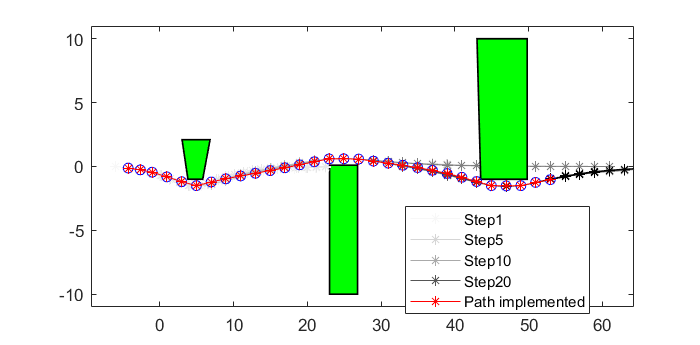
\includegraphics[width=7cm]{src/2_1_3.png}
  \label{I_ds}
  }
\label{I_V}
\caption{I-V characterstics in the subthreshold regime\\[2ex]
\protect\subref*{It_Ith} \textnormal{Tunneling and thermionic component of current}\\
\protect\subref*{I_ds} \textnormal{Total drain current}
}
\end{center}
\end{figure}


\begin{figure}[htbp]
\begin{center}
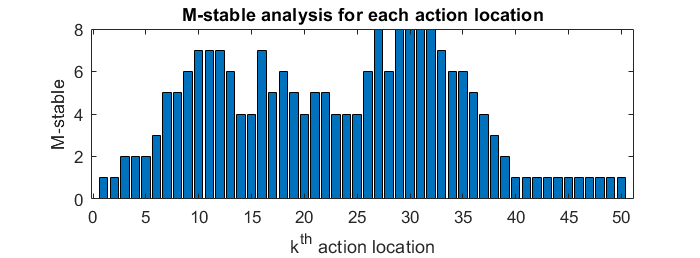
\includegraphics[width=8cm]{src/2_2_M-stable.png}
\caption{$M$-stable analysis for scenario that has initially unknown static obstacle. }
\label{fig: mpc}
\end{center}
\end{figure}

\subsection{initially unknown moving obstacle}

Similar to the previous setting, simulation is set to run for 30 time steps. The result of this scenario is shown in Fig.11 and Fig.13. In Fig.11, the robot does not know there exists the third obstacle on the right at the beginning. Once the robot detects the moving obstacle, it will also assume the obstacle is moving on a constant speed. Therefore, the robot is able to predict the future position of the obstacle and calculate the future action locations accordingly. Simulation result in Fig.11 shows that the robot avoids the obstacles successfully.

Fig.12 shows the $M$-stable analysis. It can be observed that $M$s are smaller for each action location near the $30^{th}$ one, but still, maintain at least a value of 3. This guarantees that there will not be a sudden change in the robot's motion even though the robot experienced a sudden change of the environment.

An even severe scenario is tested (Fig.13). The obstacle will change its speed at some point after detection. In the simulation, the obstacle is originally going on $y$-minus direction, after time step $t=20$, the obstacle changes its speed and starts moving on $y$-plus direction. From Fig.13 (middle plot), we can see that the robot adjust the planned trajectory to best utilize the space once it detects the speed change. The $M$-stable plot of this scenario (Fig.14) is almost exactly the same as the one with no speed change. The result indicates that as long as there is no sudden change accruing close to the current location, the robot can successfully plan a smooth trajectory.

\begin{figure}[htbp]
\begin{center}
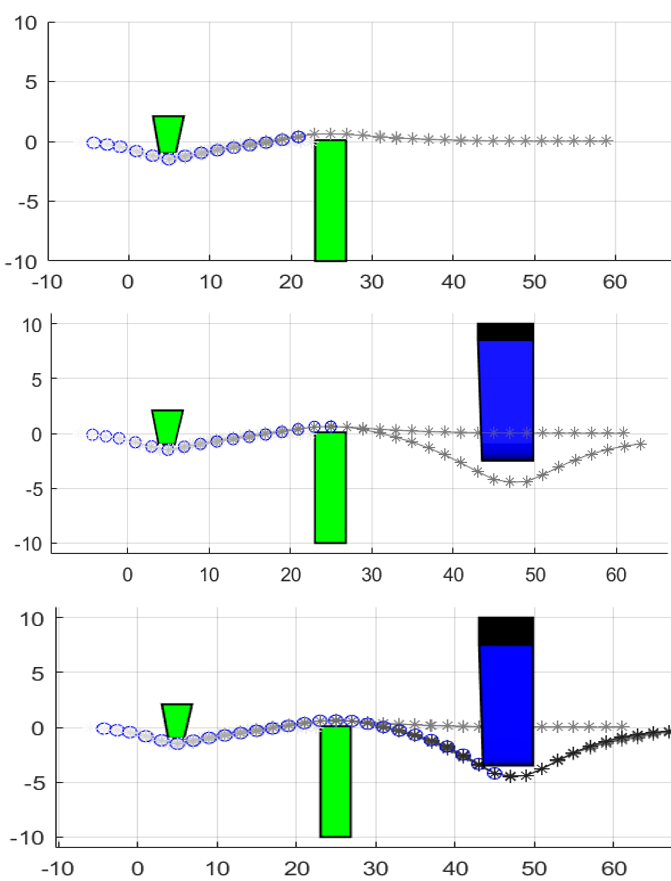
\includegraphics[width=8cm]{src/3_1_1.png}
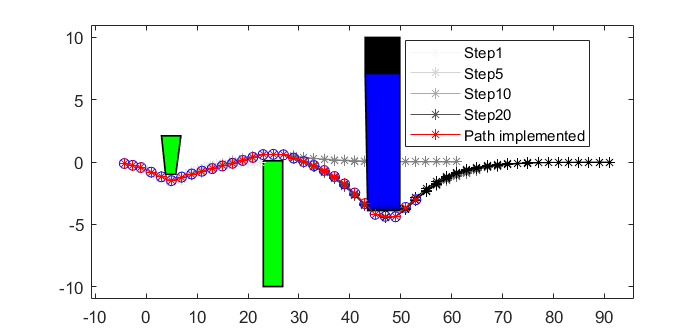
\includegraphics[width=8cm]{src/3_1_4.png}
\caption{Simulation result for scenario that has initially unknown moving obstacles. Plots are arranged going from up to down in time sequence.}
\label{fig: mpc}
\end{center}
\end{figure}

\begin{figure}[htbp]
\begin{center}
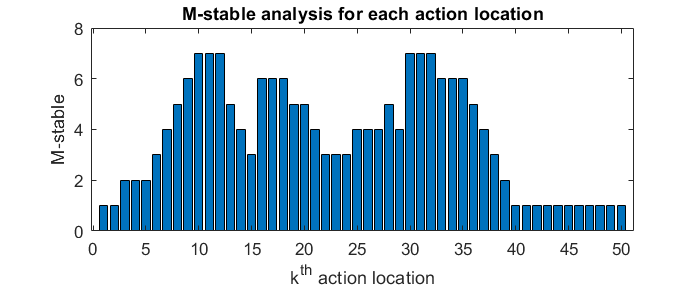
\includegraphics[width=8cm]{src/3_2_1_M-stable.png}
\caption{M-stable analysis for scenario that has initially unknown static obstacles. }
\label{fig: mpc}
\end{center}
\end{figure}


 


\begin{figure}[htbp]
\begin{center}
\includegraphics[width=8cm]{src/myfile.tex}
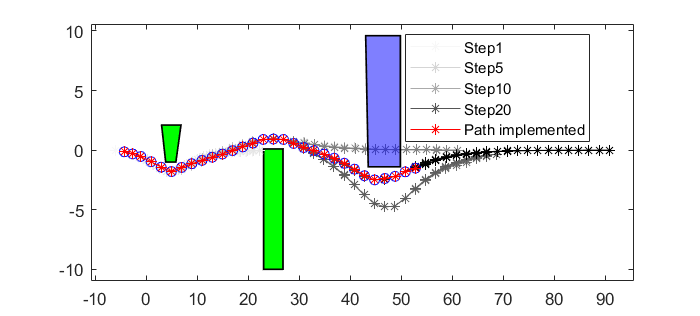
\includegraphics[width=8cm]{src/3_2_4.png}
\caption{Simulation result for scenario that has initially unknown moving obstacles (with speed change). Plots are arranged going from up to down in time sequence.}
\label{fig: mpc}
\end{center}
\end{figure}

\begin{figure}[htbp]
\begin{center}
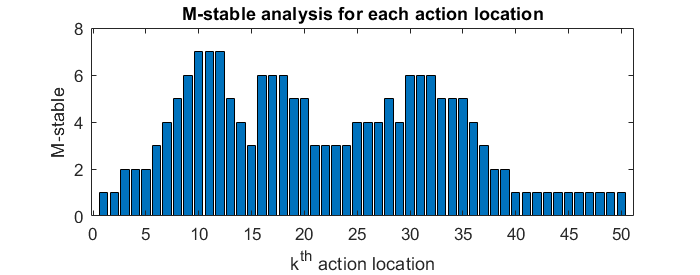
\includegraphics[width=8cm]{src/3_2_M-stable.png}
\caption{M-stable analysis for scenario that has initially unknown static obstacles (with speed change). }
\label{fig: mpc}
\end{center}
\end{figure}



\section{Conclusion}

This paper proposed a new method of analyzing stability properties for non-convex MPC implementation on mobile robots. The proposed method, $M$-stable analysis, took the difference of each action location planned at consecutive time steps in to account. We said the action location has $m$-stable property if there is smaller and smaller change between consecutive time steps after time step $k-m$. Simulation  results show that a robot implemented with CFS algorithm in MPC framework was capable of dealing with dynamic environment as long as the changes in the environment was predictable. The stability properties analyzed using $M$-stable (and also other methods for static case) is done. It was shown that the robot had decent stability properties. In the future, we will include the robot dynamics in to the problem formulation and complete the theoretical proof for $M$-stable analysis.



%\begin{ack}
%Place acknowledgments here.
%\end{ack}


 
% in the appendices.
\begin{thebibliography}{xx}  % you can also add the bibliography by hand

\bibitem[Able(1956)]{Abl:56}
N. Wu and M.C. Zhou.
\newblock Modeling and deadlock control of automated guided vehicle systems.
\newblock \emph{ IEEE/ASME Transactions on Mechatronics }, Volume: 9, Issue: 1:\penalty0 50 - 57, 2004.

\bibitem[Able(1956)]{Abl:56}
J. Wang, J. Steiber, and B. Surampudi.
\newblock Autonomous ground vehicle control system for high-speed and safe operation.
\newblock \emph{ American Control Conference }, 2008.


\bibitem[Able(1956)]{Abl:56}
F. Oleari, M. Magnani, and D. Ronzoni.
\newblock Industrial AGVs: Toward a pervasive diffusion in modern factory warehouses.
\newblock \emph{ IEEE/ICCP }, 2014.


\bibitem[Able(1956)]{Abl:56}
J.B. Rawlings.
\newblock Tutorial: model predictive control technology.
\newblock \emph{  American Control Conference }, 1999.

\bibitem[Able(1956)]{Abl:56}
D.Q. Mayne, J.B. Rawlingsb, C.V. Raob, and P.O.M. Scokaertc.
\newblock Constrained model predictive control: Stability and optimality.
\newblock \emph{  Automatica }, Volume: 36, Issue: 6:\penalty0 789 - 814, 2000.

\bibitem[Able(1956)]{Abl:56}
D. Limon, T. Alamo, and F. Salas.
\newblock On the stability of constrained MPC without terminal constraint.
\newblock \emph{   IEEE Transactions on Automatic Control }, Volume: 51, Issue: 5:\penalty0 832 - 836, 2006.

\bibitem[Able(1956)]{Abl:56}
S.S. Dughman and J.A. Rossiter.
\newblock A survey of guaranteeing feasibility and stability in MPC during target changes.
\newblock \emph{   IFAC-PapersOnLine }, Volume: 48, Issue: 8:\penalty0 813 - 818, 2015.

\bibitem[Able(1956)]{Abl:56}
L. Zhanga, S. Zhuanga, and R.D. Braatzb.
\newblock Switched model predictive control of switched linear systems:
Feasibility, stability and robustness.
\newblock \emph{  Automatica  }, Volume: 67\penalty0 8 - 21, 2016.

\bibitem[Able(1956)]{Abl:56}
A. Bocciaa, L. Grüneb, and K. Worthmannc.
\newblock Stability and feasibility of state constrained MPC without stabilizing terminal constraints.
\newblock \emph{  Systems $&$ Control Letters  }, Volume: 72\penalty0 14 - 21, 2014.



\bibitem[Able(1956)]{Abl:56}
F. Borrelli.
\newblock Stabilization of 2-D Spider Crane with Non-Convex State Constraints using MPC.
\newblock \emph{ Inderscience Enterprises Limited  }, Volume: 3, Issue: 2\penalty0 265 - 290, 2006.

\bibitem[Able(1956)]{Abl:56}
T.G. Hovgaard, L.F.S. Larsen, J.B. Jørgensen, and S. Boyd.
\newblock Nonconvex Model Predictive Control for Commercial Refrigeration.
\newblock \emph{ IFAC Proceedings Volumes  }, Volume: 45, Issue: 17\penalty0 514 - 521, 2012.

\bibitem[Able(1956)]{Abl:56}
C. Liu, C.Y. Lin, and M. Tomizuka.
\newblock The Convex Feasible Set Algorithm for Real Time Optimization in Motion Planning.
\newblock under review in \emph{ SIAM Journal on Control and Optimization}, arXiv:1709.00627, 2016.




%\bibitem[Able et~al.(1954)Able, Tagg, and Rush]{AbTaRu:54}
%B.C. Able, R.A. Tagg, and M.~Rush.
%\newblock Enzyme-catalyzed cellular transanimations.
%\newblock In A.F. Round, editor, \emph{Advances in Enzymology}, volume~2, pages
%  125--247. Academic Press, New York, 3rd edition, 1954.

%\bibitem[Keohane(1958)]{Keo:58}
%R.~Keohane.
%\newblock \emph{Power and Interdependence: World Politics in Transitions}.
%\newblock Little, Brown \& Co., Boston, 1958.

%\bibitem[Powers(1985)]{Pow:85}
%T.~Powers.
%\newblock Is there a way out?
%\newblock \emph{Harpers}, pages 35--47, June 1985.

%\bibitem[Soukhanov(1992)]{Heritage:92}
%A.~H. Soukhanov, editor.
%\newblock \emph{{The American Heritage. Dictionary of the American Language}}.
%\newblock Houghton Mifflin Company, 1992.

\end{thebibliography}
\end{document}
